
\newprob{1715330504}
{
    支架$PQ$上架了一樑橫木,如圖。横木重 \qty{300}{N}。 有一個重 \qty{600}{N} 的人從$Q$點,慢慢向右走。\bigskip
    {\par\centering
        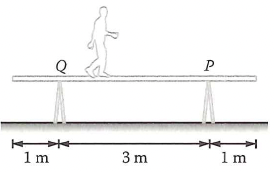
\includegraphics[width=.3\textwidth]{assets/efd30991.png}
        \par}\bigskip
    那人走到何處,橫木就會翻起?
    \begin{tasks}
        \task $P$點之右 \qty{0.5}{m}
        \task $P$點之左 \qty{0.5}{m}
        \task $P$點之右 \qty{0.75}{m}
        \task $P$點之左 \qty{0.75}{m}
    \end{tasks}
}{\mckey{C}}

\newprob{1715331378}
{
    如圖,一塊高 \qty{5}{cm} 、底長 \qty{12}{cm} 、且重量為 \qty{10}{N} 的三角木塊$ABC$放在水平面上。當一道量值 \qty{3}{N} 的施力$F$ 向左作用於 $A$ 點時,木塊開始翻側。現在如果 $F$ 指向右,其量值應為多少,方能使木塊開始翻側?\bigskip
    {\par\centering
        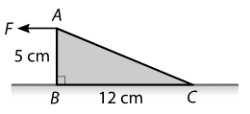
\includegraphics[width=.3\textwidth]{assets/ad661d08.png}
        \par}\bigskip
    \begin{tasks}
        \task \qty{6.2}{N}
        \task \qty{8.1}{N}
        \task \qty{16}{N}
        \task \qty{21}{N}

    \end{tasks}
}{\mckey{D}}

\newprob{1715331721}
{
    一磚勻質方塊,高 $h$ 闊$\ell$,擱在地毯上。把地毯 以加速度 $a$ 水平拉動。
    \bigskip
    {\par\centering
        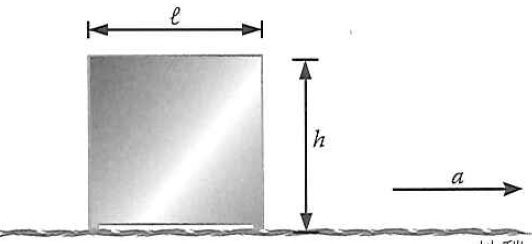
\includegraphics[width=.3\textwidth]{assets/5b765e46.png}
        \par}\bigskip
    假設方塊沒有翻側,也沒有滑移,$a$ 的最大值是 多少?
    \begin{tasks}
        \task $\dfrac{g\ell}{h}$
        \task $\dfrac{gh}{\ell}$
        \task $\dfrac{g\ell}{\sqrt{\ell^2+h^2}}$
        \task $\dfrac{g\sqrt{\ell^2+h^2}}{\ell}$
    \end{tasks}
}{A}

\newprob{1715420160}
{
    % cw sham 2019 mock 8 9
    \topalignc{\par\centering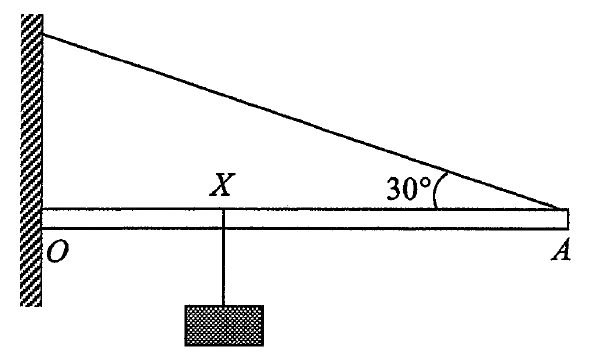
\includegraphics[width=.33\textwidth]{./img/ch3_moment_prob_2024-05-11-17-37-45.png}\par} \bigskip\par
    一個長度為 \qty{80}{cm} 的輕質剛性棒$OA$在一端$O$與牆壁鉸接。一個重量為 24 N 的物體附著在 $X$ 上,其中$OX$等於 \qty{30}{cm}。一條輕質繩子附著在$A$上,使得繩子與棒成 \dg{30}。棒保持水平。計算牆壁對棒的反作用力。
    \begin{tasks}
        \task \qty{15.6}{N}
        \task \qty{18.0}{N}
        \task \qty{21.6}{N}
        \task \qty{22.5}{N}
    \end{tasks}

}{\mckey{C}}

\newprob{1715332021}
{
    一個質量為 0.15 kg 的均勻米尺在 $P$ 點鉸接到牆上,另一端$R$則通過一根連接到$Q$點的鋼線固定在牆上, $Q$ 點位於 $P$ 點的正上方。一個質量為 0.1 kg 的方塊 $X$ 從距離 $R$ 點 30 cm 處懸掛在米尺上。米尺水平放置。求鋼線張力對$P$點產生的力矩。 \bigskip
    {\par\centering
        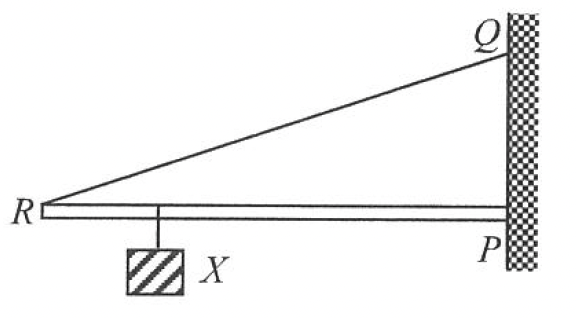
\includegraphics[width=0.33\textwidth]{assets/84e42251.png}
        \par} \bigskip
    \begin{tasks}
        \task \qty{1.42}{N.m}
        \task \qty{1.05}{N.m}
        \task \qty{0.75}{N.m}
        \task \qty{0.70}{N.m}
    \end{tasks}
}{\mckey{A}}

\newprob{1715332165}
{
一個勻質硬竿AB,以A為支軸,它由一金屬線接連牆壁上位於A點豎直上方的C點,使竿維持水平。竿上掛着負荷W。若將W逐漸從A移向B,下列哪些數量會增加?
{\par\centering
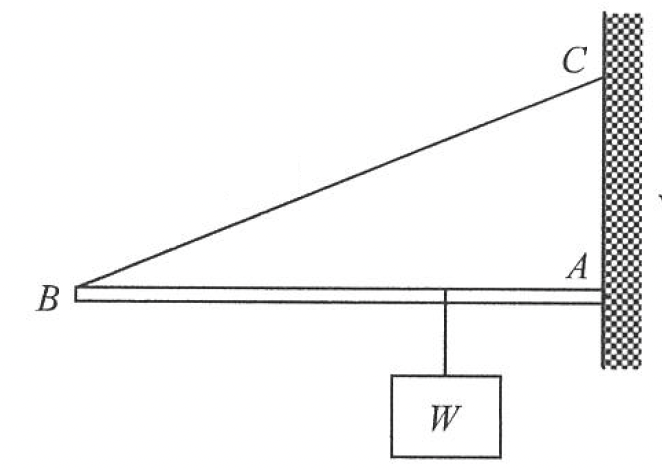
\includegraphics[width=.3\textwidth]{assets/a9b14a8d.png}
\par}
\begin{statements}
    \task 金屬線上的張力。
    \task 竿所受到的水平壓縮力。
    \task A點上的作用力的垂直分量。
\end{statements}
\begin{tasks}
    \task 只有(1)
    \task 只有(3)
    \task 只有(1)和(2)
    \task 只有(2)和(3)
\end{tasks}
}{\mckey{C}}

% \newprob{1715331830}
% {
% 一輕剛棒 $PO$ 的一端順滑地鉸接在牆上,另一端則以不能拉伸 的線接於$P$ 點正上方的$R$點。一負荷 $W$ 懸掛在棒上某點。若 棒保持水平,下列哪些改變會令線的張力增加?
% {\par\centering
% 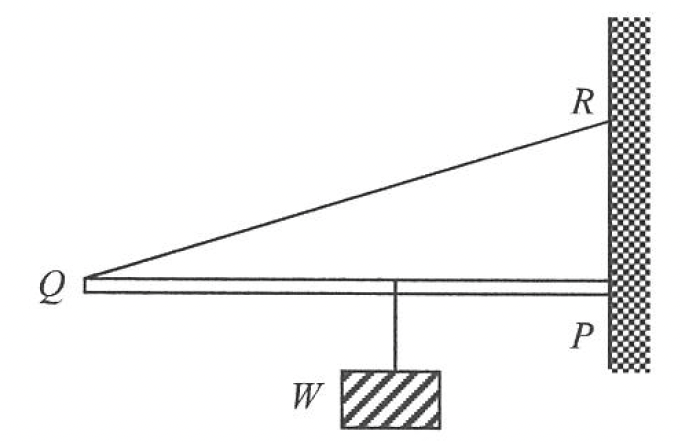
\includegraphics[width=.3\textwidth]{assets/4f96447b.png}
% \par}
% \begin{statements}
%     \task
%     將重量移向 $Q$
%     \task
%     更換較短的線,並分別接於 $PQ$ 和 $PR$ 的中點
%     \task
%     更換較長的線,並接於較 $R$ 爲高的一點
% \end{statements}
% \begin{tasks}
%     \task 只有(1)
%     \task 只有(2)
%     \task 只有(3)
%     \task 只有(1)和(2)
%     \task 只有(1)和(3)
%     \task 只有(2)和(3)
%     \task (1), (2) 和 (3)
% \end{tasks}
% }{}


\newprob{1715417908}
{
    % jointusMC p199 44
    \topalignc{\par\centering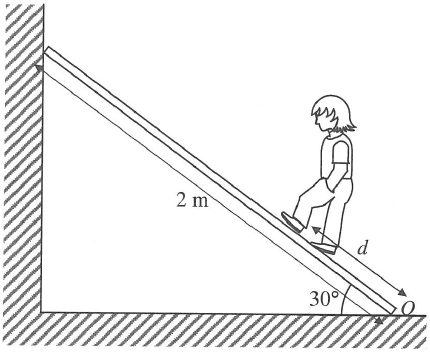
\includegraphics[width=.3\textwidth]{./img/ch3_moment_prob_2024-05-11-17-01-54.png}\par} \par\bigskip
    一個重量為 \qty{600}{N} 的男子從$O$點沿著梯子往上走,如上圖所示。牆壁是光滑的,地板是粗糙的。梯子的長度為 \qty{2}{m},梯子的重量為 \qty{500}{N} ,梯子和地板之間的最大摩擦力為 \qty{700}{N} 。他最多可以沿梯子走多遠的距離($d$),以保持梯子不會滑動?
    \begin{tasks}
        \task \qty{0.514}{m}
        \task \qty{1.03}{m}
        \task \qty{1.45}{m}
        \task \qty{2}{m}
    \end{tasks}

}{\mckey{A}}

\newprob{1715418290}
{
    % jointusMC p199 65
    以$O$為支點,以下哪個情況的合力矩量值是最大的? \bigskip
    \begin{tasks}(2)
        \task \topalign{\par\centering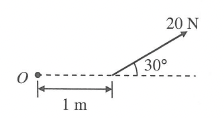
\includegraphics[width=.3\textwidth]{./img/ch3_moment_prob_2024-05-11-17-07-14.png}\par}
        \task \topalign{\par\centering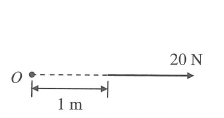
\includegraphics[width=.3\textwidth]{./img/ch3_moment_prob_2024-05-11-17-07-36.png}\par}
        \task \topalign{\par\centering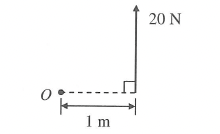
\includegraphics[width=.3\textwidth]{./img/ch3_moment_prob_2024-05-11-17-09-58.png}\par}
        \task \topalign{\par\centering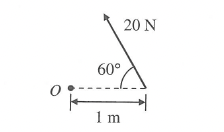
\includegraphics[width=.3\textwidth]{./img/ch3_moment_prob_2024-05-11-17-08-00.png}\par}
    \end{tasks}

}{\mckey{C}}

\newprob{1715418651}
{
    % jointusMC p199 66
    \topalignc{\par\centering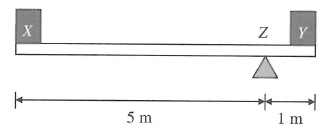
\includegraphics[width=.4\textwidth]{./img/ch3_moment_prob_2024-05-11-17-12-09.png}\par} \par\bigskip
    如上圖所示,一個質量為 2 kg 的均勻木板放在一個支撐點上。$X$和$Y$是質量分別為 2 kg和 14 kg 的物體。以下哪些陳述是\textbf{不正確}的?
    \begin{statements}
        \task 木板處於平衡狀態。
        \task 支撐點對木皮所施加的力為 \qty{20}{N}
        \task 如果現在在$Z$點對木板施加向上的力,木板將繞著$Z$點旋轉。
    \end{statements}
    \begin{tasks}
        \task 只有(1)和(2)
        \task 只有(1)和(3)
        \task 只有(2)和(3)
        \task (1), (2) 和 (3)
    \end{tasks}
}{\mckey{C}}

\newprob{1715419124}
{
    % jointus p114 75
    \topalignc{\par\centering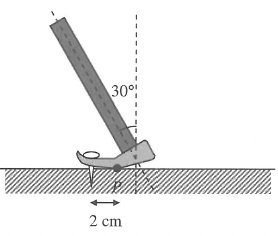
\includegraphics[width=.35\textwidth]{./img/ch3_moment_prob_2024-05-11-17-18-48.png}\par}\bigskip
    一個男人使用一把質量可忽略不計的錘子從一個木塊的表面上取出一個質量為 5 g 的釘子。錘子的手柄長度為 25 cm,如圖所示,與垂直方向成 \dg{30}。當釘子即將被取出時,錘子與木塊接觸的唯一點為$P$。如果木塊對釘子的平均摩擦力為 15 N,求取出釘子所需的最小力。
    \begin{tasks}
        \task \qty{0.01}{N}
        \task \qty{0.02}{N}
        \task \qty{1.1}{N}
        \task \qty{1.2}{N}
    \end{tasks}
}{\mckey{D}}

\newprob{1715419567}
{
    % jointus 115 76
    \topalignc{\par\centering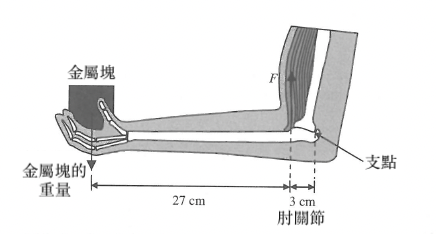
\includegraphics[width=.4\textwidth]{./img/ch3_moment_prob_2024-05-11-17-27-51.png}\par} \bigskip
    一個男孩用他的左手拿著一個重量為 20 N 的金屬塊,如圖所示。他的前臂(包括手)的重量$W$ 作用於他的肘關節和金屬塊之間。他的肱二頭肌對前臂施加向上的力為$F$。以下哪些陳述是\textbf{不正確}的?
    \begin{statements}
        \task 如果男孩想要將金屬塊舉起,且他的前臂(包括手)的重量是 10 N,則$F$的最小量值為 240 N。
        \task 他的手臂充當一個力量放大器。
        \task 如果金屬塊靠近肘關節放置,肱二頭肌需要施加更大的力。
    \end{statements}
    \begin{tasks}
        \task 只有(1)和(2)
        \task 只有(1)和(3)
        \task 只有(2)和(3)
        \task (1), (2) 和 (3)
    \end{tasks}
}{\mckey{D}}

\newprob{1715420450}
{
    % jointus 113 74
    \topalignc{\par\centering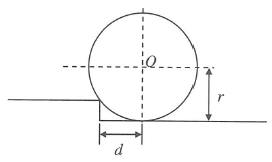
\includegraphics[width=.4\textwidth]{./img/ch3_moment_prob_2024-05-11-17-41-10.png}\par} \par\bigskip
    上圖顯示了一個帶有軸$O$、半徑$r$和質量$m$的重型滾筒。如果要將滾筒拉上臺階,最小所需力$F_1$是多少?如果力的方向必須水平於地面且通過$O$點,所需的力$F_2$是多少?
    \begin{tasks}
        \task [] $\mathbf{F_1}$ \tab\tab $\mathbf{F_2}$\vspace{.8em}
        \task $\dfrac{mg}{2}$ \tab\tab $\dfrac{mgd}{r}$
        \task $\dfrac{mg}{2}$ \tab\tab $\dfrac{mgd}{\sqrt{r^2-d^2}}$
        \task $\dfrac{mgd}{2r}$ \tab\tab $\dfrac{mgd}{r}$
        \task $\dfrac{mgd}{2r}$ \tab\tab $\dfrac{mgd}{\sqrt{r^2-d^2}}$
    \end{tasks}

}{\mckey{D}}